%!TEX root = ../dokumentation.tex

	\chapter{Hindernisse}
	Die Interaktion mit seiner Umwelt ist ein essentieller Teil in der Anwendung autonomer Systeme. Besonders der Sicherheitsaspekt spielt hier eine primäre Rolle. Die Akzeptanz der potentiellen Nutzer wäre stark beeinträchtigt wenn die Unversehrtheit von umstehenden Lebewesen und Gegenständen nicht sichergestellt werden kann. Die Komplexität bei Umweltinteraktion zeigt sich besonders beim Auftreten dynamischer Events. Ein Beispiel hierfür ist das Erscheinen von Hindernissen im Bewegungsraum einer mobilen Plattform. Um auf solche Ereignisse angemessen zu reagieren müssen dynamische Objekte erkannt, verfolgt und identifiziert werden. Bei der Entkopptlung der Intelligenz vom Roboter selbst, eröffnet sich ein weiteres Problem. Die Unterscheidung zwischen einem dynamischen Objekt und der mobilen Plattform. Im folgenden \underline{Kapitel} soll ein Konzept für ein solches Szenario erarbeitet und umgesetzt werden.
%	\begin{itemize}
%	\item interaktion mit Umwelt essentiell für autonomes System
%	\item Sicherheitsaspekt kein Verletzungsrisiko für umstehende Lebewesen durch Einsatz eines autonomen systems
%	\item Wo besteht hier die Schwierigkeit
%	\item Objekte erkennen
%	\item Objekte verfolgen
%	\item Objekte identifizieren
%	\end{itemize}
		\section{Definition von Hinderniss}
		Die Definition lautet wie folgt: \"Etwas, was das direkte Erreichen eines Ziels, das Weiterkommen be- oder verhindert.\". \cite{duden-hinderniss} Dabei wird offengelassen welche Ursache das Hinderniss sein kann, Gegenstände und Lebewesen werden hier nicht unterschieden, somit wird im weiteren Verlauf lediglich die neutrale Form Objekt genutzt. Genauer von Objekten welche den Bewegungsraum der Mobilen Plattform betreten bzw. sich bereits darin befinden. Zusätzlich müssen Objekte anhand ihres Verhaltens Klassifiziert werden. Dies ist notwendig da nicht auf jede Situation mit dem selben Vorgehen reagiert werden kann. Dadurch entsteht die Möglichkeit auf Basis der definierten Klassen eine Fallunterscheidung mit dafür angepassten Reaktionsroutinen zu entwerfen.
%		\begin{itemize}
%		\item Ein Objekt was sich im Bewegungsraum der Mobilen Plattform befindet.
%		\item Unterscheidung unterschiedlicher Hindernisse bzw Objekte durch Klassifizierung.
%		\item Notwendig da nicht auf jede Situation gleich reagiert werden kann = F allunterscheidung. Klassifizierung Werkzeug für Fallunterscheidung.
%		\end{itemize}
		
		\begin{itemize}
		\item dynamisches Objekt = Lebewesen oder Gegenstand welches den Bildbereich der Kamera betritt. Bewegt sich kontinuierlich auf einem festen Pfad durch den Bewegungsraum der Plattform.
		\item statisches Objekt = Lebewesen oder Gegenstand welches in den Bewegungsraum der Plattform betritt und dort an einem festen Punkt verweilt.
		\item chaotisches Objekt = Lebewesen oder Gegenstand welches ohne vorhersehbares Muster im Bewegungsraum der Plattform umherwandelt, und in unregelmäßigen Abständen für eine undefinierbare Zeit an einem fixen Punkt verweilt.
		\item \underline{Blitz} Objekt = Lebewesen oder Gegenstand welches den Bewegungsraum der Mobilen Plattform nur sehr flach durchstreift i.e. den Bewegungsraum nicht tief betritt oder ihn lediglich tangiert, aber dennoch von der Raumüberwachung erfasst wird.
		\end{itemize}
		
		
		\section{Objekte erkennen}
		Die Grundlage für jede Interaktion mit der Umgebung, unabhängig davon ob nun von einem Roboter oder einem Lebewesen gesprochen wird, bildet die Voraussetzung zu Erkennen und zu Verstehen was darin vorgeht. Bei Lebewesen wie Robotern geschieht dies über die Audio-Visuellen Schnittstellen des Körpers bzw. des Systems.
%		\begin{itemize}
%			\item Grundlage für Interaktion = erkennen
%			\item Erkennen Anhand welcher Informationen? Arbeitsgrundlage?
%			\item mehrere Ansätze zum Lösen des Problems
%			\item Nutzung von OpenCV
%			\item mit und ohne Farben möglich
%			\item Farbe verfolgt Object anhand der Bewegung von Farbwerten in jedem Pixel
%	%		\item findContours
%	%		\item inRange
%			\item ohne Farbe
%			\item Sequential Images
%		\end{itemize}
		\subsection{Konzeptionelle Lösungsansätze}
		Der Grundsätzliche Ansatz besteht darin die Umgebung mit einem Bildsensor zu überwachen und Veränderungen sichtbar zu machen und zu analysieren. Dies geschieht durch den Abgleich von Inhalten über eine Serie von Bildern. Dieses Verfahren wird in einigen Publikationen als Frame-Analysis bezeichnet. Die Unterschiede der implementierten Vertreter dieses Verfahrens liegen in den beobachteten Merkmalen der Bilder. Im Verlauf des Projekts wurden drei Varianten verglichen. Für die Implementierung wurde OpenCV genutzt. Beweggründe für diese Entscheidung können dem Theoriekapitel über OpenCV entnommen werden.\\
		\textbf{(ADD) Verweiss auf OpenCV-ref (ADD)}
		\subsection{Sequential Images}
		Eine Variante lautet \textit{sequential images}, dt. \textit{auf einander folgende Bilder}. Dabei wird eine Folge von Bildern, im Regelfall zwei $f_i$ \& $f_i+1$, im gesamten verglichen. Eine Möglichkeit dies zu tun besteht darin für jeden Pixel $p_xy$ der beiden Bilder die Differenz der Grauwerte zu erzeugen. Grauwerte deshalb da \textit{sequential images} monochrome bzw. Graufstufenbilder als Eingabe erfordern. Graustufenbilder eignen sich hierfür im Gegensatz zu Farbbildern aufgrund der Beschränkung auf 2 Maxima, schwarz und weiß, mit $n$ vielen (grauen) Zwischenwerten. Dadurch laesst sich die Differenz durch eine simple Subtraktion der Grauwerte erreichen. Das RGB Farbmodell hingegen verfügt über 8 Maxima, von denen 6 Maxima jeweils über eine Komplementärefarbe innerhalb des Farbmodells verfügen. Dies erschwert die Differenzbildung da nur in bestimmten Fällen durch eine Subtraktion der vorhandene Farbwert neutralisiert wird. Stattdessen würde man in vielen Fällen lediglich einen anderen Farbwert erhalten. Das Ziel der Differenzbildung besteht jedoch darin die gemeinsamen Merkmale die in beiden aufeinander folgenden Bildern auftauchen zu entfernen, und nur die einzigartigen Merkmale des nachfolgenden Bildes zu bewahren.\\
		Sind die Grauwerte $g_p(f_i)$, $g_p(f_i+1)$ von Pixel $p_xy$ in $f_i$ und $f_i+1$ identisch wird der Wert für diesen Pixel auf 0 (schwarz) gesetzt. Dabei handelt es sich um den Idealfall. In der reellen Anwendung dieses Verfahrens werden die Werte nur stark reduziert da durch die Dynamik der Lichtverhältnisse die Grauwerte des Pixels zwar nur marginal dafür allerdings konstant schwanken und dadurch die Wahrscheinlichkeit für das Eintreffen des Idealfalls $g_p(f_i)$ = $g_p(f_i+1)$ nur sehr gering ist.
		
		\textbf{(ADD)referenz und differenzbild(ADD)}
		
%		\begin{itemize}
%		\item Graustufenbild, monochrom
%		\item vergleicht Bild$f_0$ mit Nachfolger$f_1$
%		\item dabei wird für jeden Pixel die absolute Differenz gebildet.
%		\item Sind die Werte$w_i(f_0)$, $w_i(f_1)$ von Pixel$p_xy$ in $f_i$ und $f_i+1$ identisch wird der Wert für diesen Pixel auf 0(schwarz) gesetzt. Dabei handelt es sich um den Idealfall. In der reellen Anwendung dieses Verfahrens werden die Werte nur stark reduziert da durch die Dynamik der Lichtverhältnisse die Grauwerte des Pixels zwar nur marginal dafür allerdings konstant schwanken und dadurch die Wahrscheinlichkeit für das Eintreffen des  Idealfalls $w_i(f_0)$ = $w_i(f_1)$ nur sehr gering ist.
%		\item Durch dieses Verfahren werden dem Informationsgehalt die Gemeinsamkeiten beider Bilder entzogen, und nur die Veränderungen von $f_0$ zu $f_1$ verbleiben.
%		\item dadurch bekommt man ein Differenzbild welches die geänderten Pixel isoliert hervorhebt, was das erkennen dynamischer Objekte prinzipiell stark vereinfacht.
%		\end{itemize}
	
		\subsection{find Contour}
		Anders als \textit{sequential images} arbeitet \textit{find contour} mit Farbbilden. Die Grundmechanik besteht darin den Verlauf von Farbwerten zu verfolgen. Hierbei werden zwei Arten der Farbwertänderung detektiert. Beim Ausbreiten nimmt ein Pixel $p_i$  den Farbwert seines direkten Nachbarn an $C(P_i) = C(P_i+1)$. Das zweite Merkmal wird Wandern genannt. Hier wechselt der Farbwert von Pixel $P_i$ zu $P_i+1$, dabei nimmt $P_i$ einen anderen Farbwert an $C(P_i+1(f_1)) = C(P_i(f_0))$. Im Gegensatz zu \textit{sequential images} detektiert \textit{find contours} lediglich die Außenkanten - Konturen eines Objekts, dabei erzeugt das Ausbreiten die Vorderseite und Wandern die Rückseite des Objekts. In einigen Implementierungen werden Farbgruppen statt einzelnen Farbwerten genutzt, um die Funktionalität gegenüber Einwirkungen von Lichtquellen Robuster zu gestalten. Die Farbgruppierung enthält einen Referenzwert und weitere Werte ähnlicher Farben. Dadurch wird ein gewisser Toleranzbereich geschaffen, der unterschiedlich starke Beleuchtung oder beispielsweise Designfenster mit partieller Colorverglasung ausgleichen kann.
		
%		\begin{itemize}
%		\item RGB Bild
%		\item verfolgt die Farbänderung jedes Pixels mit Fokus auf Farbwert
%		\item sequential images legt Fokus auf Änderung im Allgemeinen = Änderung Grauwert bedeutet Änderung im Raum, detektiert Objekte im Ganzen
%		\item benachbarter Bildpunkt nimmt Farbe an(Ausbreiten), $C(P_i) = C(P_i+1)$.
%		\item Farbwert wechselt von Pixel $P_i$ zu $P_i+1$, dabei nimmt $P_i$ einen anderen Farbwert an(Wandern). $C(P_i+1(f_1)) == C(P_i(f_0))$
%		\item detektiert Außenkante Konturen engl. contour von Objekten dabei Ausbreiten = Forderseite des Objekts. Wandern = Rückseite des Objekts
%		\item in einigen Implementierungen werden statt einzelnen Farbwerten Farbgruppen gebildet, um die Funktionalität gegenüber Einwirkungen von Lichtquellen Robuster zu gestalten. Durch die Farbgruppierung wird letztendlich ein Referenzwert gewählt und weitere ähnliche Werte hinzugefügt um eine Tolleranz zu erreichen.
%		\end{itemize}

		\begin{figure}[H]
		\centering
		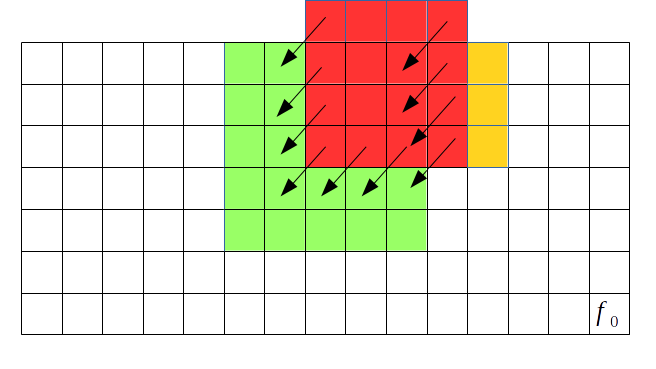
\includegraphics[width=0.7\linewidth]{../media/find-contours-spread-f0}
		\caption{Visualisierung von Ausbreiten und Wandern, erster Frame $f_0$. Die Vektoren geben die Bewegung des quadratischen Objekts an.}
		\label{fig:find-contours-spread-f0}
		\end{figure}
		\begin{figure}[H]
		\centering
		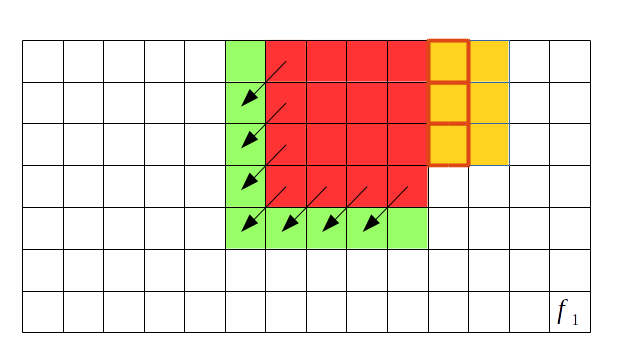
\includegraphics[width=0.7\linewidth]{../media/find-contours-spread-f1}
		\caption{Visualisierung des zweiten Frames $f_1$. Besonderes Augenmerk sollte auf das Weiterziehen der rechten Kante des roten Quadrats und dem damit verbundenen Farbwechsel der zuvor roten Pixel, verdeutlicht durch die orange Umrandung.}
		\label{fig:find-contours-spread-f1}
		\end{figure}


%		\subsection{Direkter Informationsgewinn aus Tiefenbildern}
					
		\subsection{Implementierung V1}
		Für die Implementierung der Objekterkennung wurde das \textit{sequential images} Verfahren angewandt. Der Grund hierfür war die Idee, direkt die Tiefenbilder der Kinect zu verwenden, da diese schon im 13-Bit Mono Format vorliegen. Die Funktionalität ist in einen ROS node eingebettet. Das Erzeugen des Differenzbildes wird mit der \textit{absdiff} Funktion der OpenCV-library erreicht. Dafür müssen zunächst die Bilddaten der Kinect aus dem ROS eigenen \textit{imageConstPtr}-Format in das von OpenCV verwendete \textit{CvImagePtr}-Format gewandelt werden. Hierfür wird die Konverter middleware cvBridge genutzt. \textbf{(ADD)Verweiß auf cvBridge in Vorarbeiten(ADD)}\\
		
		\begin{lstlisting}[caption=imageCallback Funktion des Objekt-Erkennungs nodes, label=imageCallback-V1, title=imageCallback-V1, language=C++]
		void imageCallback(const sensor_msgs::ImageConstPtr& image)
		{
		sensor_msgs::ImageConstPtr imageInRos;
		imageInRos = image;
		
		cv_bridge::CvImagePtr imageInCV = cv_bridge::toCvCopy(imageInRos);
		
		Mat matNow = imageInCV->image;
		
		if(firstrun == 1){
		matMinusOne = matNow;
		firstrun = 0;
		}
		
		absdiff(matNow, matMinusOne, imageDiff);
		matMinusOne = matNow;
				
		imshow("view_diff", imageDiff);
		}
		\end{lstlisting}
		\begin{itemize}
		\item Zeile 6: Konvertierung vom Datentyp imageConstPtr (ROS) zu CvImagePtr (OpenCV).
		\item Zeile 8: Kopieren der Bilddaten des aktuellen Frames in eine Mat-Speicherzelle. Vorbereitung für die Differenzenbildung, absdiff benötigt nur die Bilddaten (Mat-Datentyp). CvImagePtr enthalten noch zusätzliche Meta-Informationen über den aktuellen Frame. Mehr Details können den Datentypenbeschreibungen am Ende dieses Kapitels entnommen werden.
		\item Zeilen 10 bis 13: Während des Initialdurchlaufs liegt noch kein Vorgänger-Frame vor, dadurch wird in die Speicherzelle matMinusOne der aktuelle Frame geladen.
		\item Zeile 15: Bilden des Differenzframes mit \textit{absdiff}. Die Funktionsattribute sind der aktuelle Frame, der Vorgängerframe sowie eine Speicherzelle des Typs Mat für die erzeugte Differenz.
		\item Zeile 16: Hier wird der aktuelle Frame in die Speicherzelle \textit{matMinusOne} geladen, um bei der nächsten Iteration als Vorgängerframe zur Verfügung zu stehen.
		\item Zeile 18: imshow gibt den Inhalt einer übergebenen Mat-Speicherzelle (hier das Differenzbild - \textit{imageDiff}) in einem Anzeigefenster mit dem Titel \textit{view\_diff} aus. Dies dient nur zu Debug-Zwecken um äußere Einflüsse wie die Ausleuchtung des Raumes und natürliches Licht und deren Auswirkungen auf das Differenzbild zu beobachten.
		\end{itemize}
		
		Die Beobachtung der ersten Implementierung zeigte dass das Tiefenbild der Kinect nicht für das \textit{sequential images}-Verfahren geeignet ist. Das sehr starke Rauschen im Tiefenbild verhindert eine saubere Differenzbildung. Das Rauschen konnte auch durch Anwenden des Gauß-Filters nicht genug gemindert werden. Dies war der Anlass für eine zweite Implementierung.
		
		\begin{figure}[H]
		\centering
		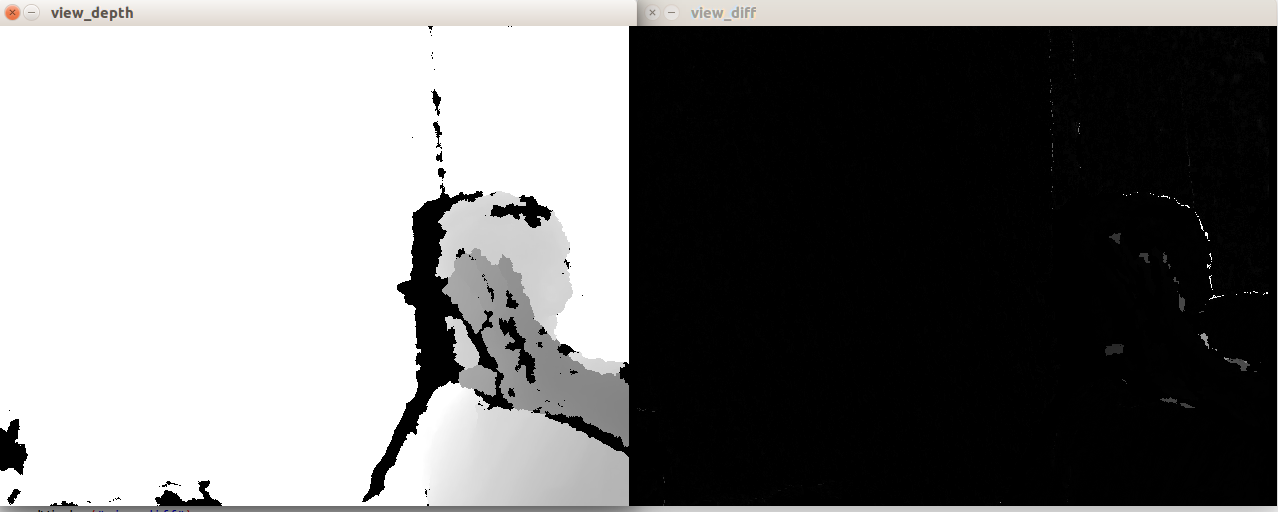
\includegraphics[width=0.7\textwidth]{../media/depth-diff}
		\caption{Darstellung des Tiefenbildes links und des Differenzbildes rechts. Durch das Rauschen im Tiefenbild wird die Differenz stark beeinträchtigt und praktisch nicht Nutzbar.}
		\label{fig:depth-diff}
		\end{figure}

		
%		\begin{itemize}
%		\item Warum "sequential images"; idee war Tiefenbilder zu verwenden da Tiefe = Graustufe
%		\item 
%		\end{itemize}
%		\begin{itemize}
%				\item Implementierung als ROS subscriber-node lauscht auf camera-depth-image topic von freenect\_launch
%				\item OpenCV Fkt absdiff(absolute differential); braucht graustufe; benötigt 2 Bilder als eingabe liefert differenzielles Bild entweder in Bild1 zurück oder in übergebenen Ausgabespeicher
%				\item ros eigene sensor-msgs images Nachrichten in OpenCV format bringen
%				\item wo liegt der Unterschied?
%				\item in CMakelists.txt -> add\_executable + add\_library
%				\item anpassungen bezüglich graustufenbilder in image\_converter.cpp
%				\item Rauschen sehr instabil, Gauß Filter keinen Effekt
%				\item Tiefenbilder zu Abhängig von Beleuchtung; schlecht
%		\end{itemize}

						
		\subsection{Implementierung V2}
		Die zweite Implementierung nutzt statt der Tiefenbilder das monochrome Bild des Kinect RGB-Sensors. Da RGB-Sensoren keine Bilder auf Basis eines IR-Meshes erzeugen, sondern lediglich die vorhandene Umgebungsbeleuchtung nutzen, weisen die damit erzeugten Bilder nahezu keine Interferrenzmuster durch natürliche IR-Strahlung auf. Der Differenzbildende Prozess hat sich im Vergleich zur erste Implementierung nicht verändert. Jedoch wurden Techniken zur Nachbearbeitung des Differenzbildes eingesetzt um das Ergebnis zu optimieren. Zum einen wurde die Threshold-Funktion von OpenCV verwendet welche den Kontrast des Bildes erhöht, um die Kanten sich bewegender Objekte deutlicher vom Hintergrund abzuheben. Anschließend wurde das durch die Threshold-Funktion entstandene Rauschen mit der Anwendung des Blur-Filters gemildert.\\
%		\begin{itemize}
%		\item rgb to mono weniger interferenz durch natürliches Licht; automatisch stabiler
%		\item threshold sorgt für verteilung auf 2 Maxima, schwellwert-operation $I_p > \text{threshold} = \text{weiß}; I_p < \text{threshold} = \text{schwarz}$
%		\item abprüfen ob Frame weiße Elemente enthält
%		\item publish stop auf robotino-handler
%		\end{itemize}
		\textbf{(ADD)PAP und Codeschnipsel(ADD)}
		\newpage
		\begin{lstlisting}[caption=imageCallbackV2 Funktion des Objekt-Erkennungs nodes, label=imageCallback-V2, title=imageCallback-V2, language=C++]
		void imageCallback(const sensor_msgs::ImageConstPtr& image)
		{
		sensor_msgs::ImageConstPtr imageInRos;
		imageInRos = image;
		
		cv_bridge::CvImagePtr imageInCV = cv_bridge::toCvCopy(imageInRos);
		
		Mat matNow = imageInCV->image;
		if(firstrun == 1){
		matMinus1 = matNow;
		firstrun = 0;
		}
		
		absdiff(matMinus1, matNow, imageDiff);
		matMinus1 = matNow;
		Mat imageThresh;
		threshold( imageDiff, imageThresh, 10, 255,0);
		Mat imageBlur;
		blur(imageThresh,imageBlur,cv::Size(10,10));
		
		    cv::imshow("view_mono", matNow);
		    cv::imshow("view_diff", imageDiff);
		    cv::imshow("view_thresh", imageThresh);
		    cv::imshow("view_blur", imageBlur);
		}
		\end{lstlisting}
		
		\begin{itemize}
				\item Zeile 17: Anwendung der Threshold Funktion auf das erzeugte Differenzbild. Threshold ist eine Schwellwert Operation. Sie korrigiert die Farbwerte für jeden Pixel in Abhängigkeit seines aktuellen Wertes. Ist sein Farbwert unterhalb des Schwellwert wird er auf den Minimalwert reduziert. Liegt seine Intensität oberhalb des Schwellwertes wird er auf den Maximalwert korrigiert. Die ersten beiden Attribute geben die Speicherzellen für das Eingabe bzw. Ausgabe Bild an. Der dritte Übergabewert ist der Schwellwert selbst. Der Maximalwert auf den die Werte $>$ Schwerllwert gesetzt werden sollen, ist das vierte Attribut. Zuletzt muss der Operations-Typ vorgegeben werden. Hier wurde mit $0$ die \textit{Binary}-Operation benutzt welche das oben beschriebene Verhalten triggert.
				\item Zeile 19: Die Blur-Funktion der OpenCV-library kann zum Filtern von Rauschen genutzt werden. Der Effekt ähnelt dem Weichzeichnen, was einen verschmierenden Effekt hat. Dies wird durch das Anwenden eines Filters auf jeden Bildpunkt erreicht. Hier wurde der \textit{normalized box filter} genutzt. Er berechnet für jeden Pixel den Durchschnitt der Farbwerte seiner Nachbarpixel, und gleicht den eigenen Farbwert daran an. Das Attribut cv:Size() gibt den Kern(Nullvektor einer Matrix) des Filters an.
		\end{itemize}
		\cite{cv-filter}
		\cite{unger13}
		\cite{cv-thresh}
				
		\begin{figure}[H]
		    \subfigure[monochrom]{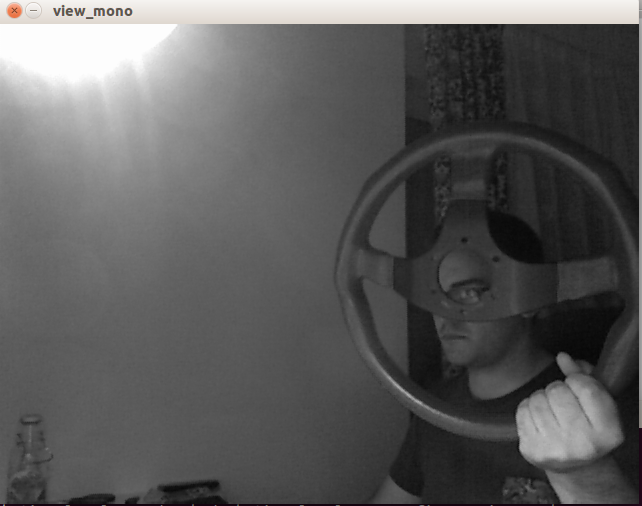
\includegraphics[width=0.4\textwidth ]{media/image-mono.png}}
		    \subfigure[Differenz]{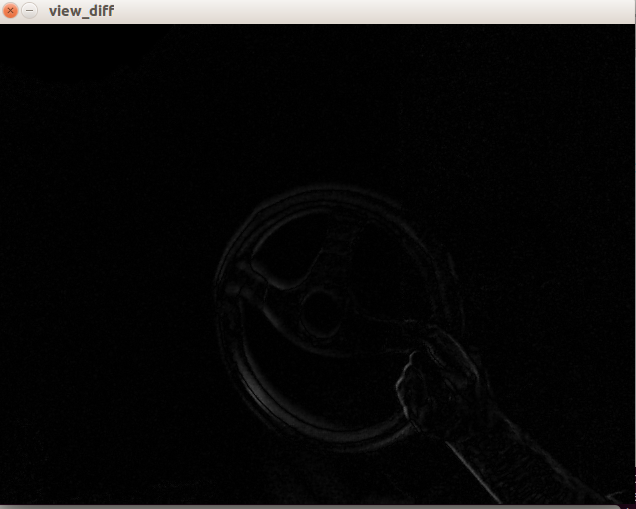
\includegraphics[width=0.4\textwidth]{media/image-diff.png}}
		\caption{Darstellung des monochromen Ursprungsbild der Kinect, rechts davon das damit erzeugte Differenzbild.}
		\end{figure}
		
		\begin{figure}[H]
				    \subfigure[Threshold]{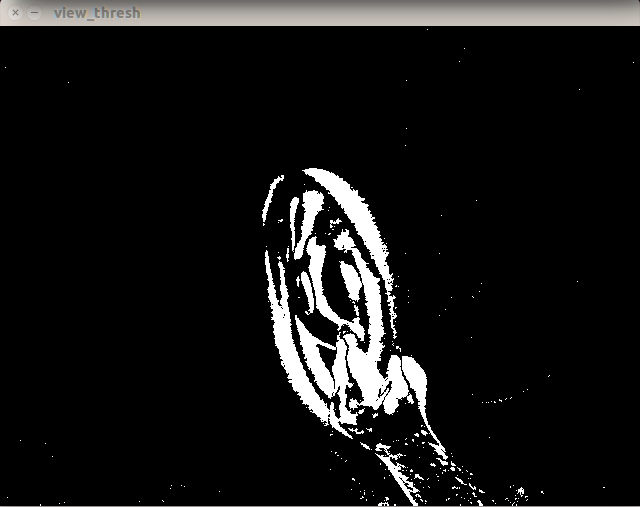
\includegraphics[width=0.4\textwidth ]{media/image-thresh.png}}
				    \subfigure[Blur]{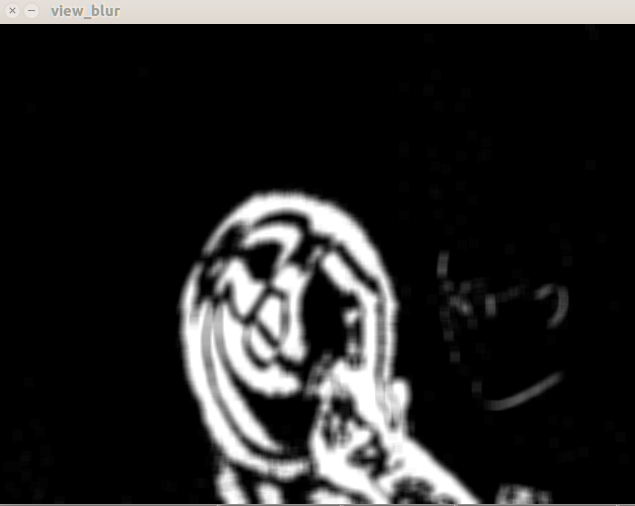
\includegraphics[width=0.4\textwidth]{media/image-blur.png}}
				\caption{Die Linke Abbildung zeigt das Ergebnis der Threshold-Funktion welche auf das Differenzbild angewendet wurde. Die Filterung des Threshold-Bilds mit der Blur-Funktion ist auf der rechten Seite dargestellt. Zu Beachten ist das Fehlen der Rauschanteile.}
				\end{figure}
			
		
		\subsection{Unterschiede Bilddatentypen}
		Die folgenden Tabellen sollen die Unterschiede der beiden oben erwähnten Datentypen verdeutlichen.
\begin{table}[H]
\begin{tabular}{|l|l|l|}
\hline \rule[-2ex]{0pt}{5.5ex} Name & Inhalt & Basisdatentyp \\ 
\hline \rule[-2ex]{0pt}{5.5ex} header & Informationen über Frame & std\_messages \\ 
\hline \rule[-2ex]{0pt}{5.5ex} height & Framehöhe & uint32\\ 
\hline \rule[-2ex]{0pt}{5.5ex} width & Framebreite & uint32\\  
\hline \rule[-2ex]{0pt}{5.5ex} encoding & Bildkodierung & String\\  
\hline \rule[-2ex]{0pt}{5.5ex} is\_bigendian & least significant bit & uint8\\ 
\hline \rule[-2ex]{0pt}{5.5ex} step & Zeilenlänge in Bytes & uint32\\ 
\hline \rule[-2ex]{0pt}{5.5ex} data[] & Bildpunkte 2D-Array (step * Zeilenanzahl) & uint8\\ 
\hline
\end{tabular}
\caption{Tabellarische Darstellung des ROS eigenen Datentyps \textit{ImageConstPtr}.} 
\end{table}
Der Datentyp des headers std\_messages ist selbst ein synthetischer Datentyp, er kann wiederum Werte der Typen \textit{int, String, double} enthalten.
\begin{table}[H]
\begin{tabular}{|l|l|l|}
\hline Name & Inhalt & Basisdatentyp\\ 
\hline source & Bildquelle & String\\
\hline encoding & Bildkodierung & String\\
\hline image[] & Bildpunkte als 2D-Array $P_i(X/Y)$ & Mat\\
\hline
\end{tabular}
\caption{Tabellarische Darstellung des OpenCV Datentyps \textit{CvImagePtr}.}
\end{table}
Der Datentyp Mat ist ein Array des Typs \textit{unsigned int 8}
 				 
		
\section{Objekte Identifizieren}
Die herkömmliche Herangehensweise einen Roboter mit visueller Wahrnehmung auszustatten besteht darin, direkt auf dem Chassis des Roboters eine Kamera zu verbauen. Durch die Trennung von Roboter und optischen Sensoren eröffnet sich ein zusätzliches Problem. Da der Roboter sich innerhalb des Bildbereichs bewegen soll wird er zwangsläufig selbst als mobiles Hindernis wahr genommen. Um diesen Fall zu umgehen müssen alle sich bewegenden Elemente des Bilds identifiziert werden. Die grundsätzliceh Aufgabe besteht nun darin die mobile Plattform von Objekten zu unterscheiden. Das Open-Source Projekt \textit{Find\_Object} enthält die hierfür benötigten Funktionen und wurde bereits in die ROS Infrastruktur integriert.
%\begin{itemize}
%\item Herkömmliche Herangehensweise Kamera auf dem Roboter
%\item Durch Trennen der Kamera vom Roboter entsteht ein zusätzliches Problem; Roboter bewegt sich selbst im Bewegungsraum; Wie mache ich dem System bekannt dass %es sich nicht um ein Hindernis sondern um den Roboter selbst handelt.
%\item darum Lösung zum identifizieren von Objekten benötigt
%\item findobjekt-2D bietet benötigte Funktionalitäten
%\item bereits in ROS integriert.
%\end{itemize}

	\subsection{Identifizieren der mobilen Plattform}
	Die Identifikation von Objekten mit \textit{find-object} erfolgt durch das Registrieren der gesuchten Objekte. Die Registrierung wird über die GUI durchgeführt. Dazu wird zunächst ein Foto des Objekts angefertigt. Das Programm ermittelt nun Markante Punkte innerhalb des Bildes. Durch das Zuschneiden des Bildes auf die Außenmaße des Objekts, bekommt man ein Template des registrierten Objekts. Das eigentliche Idntifizieren von Objekten innerhalb eines Frames erfolgt durch das abgleichen seiner markanten Punkte mit denen des Objekttemplates.\newline
	
	\begin{figure}[H]
	\centering
	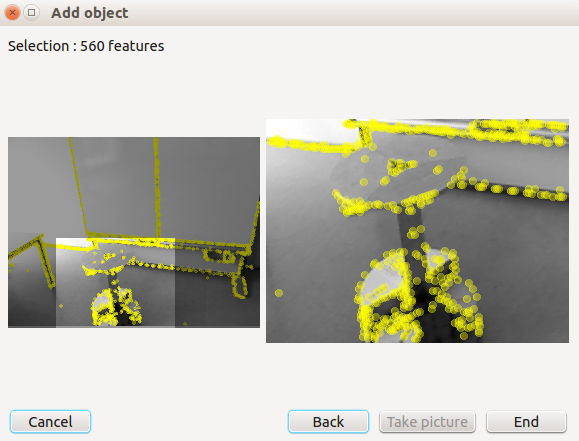
\includegraphics[width=0.7\linewidth]{../media/add-object-2}
	\caption[template-addobject]{Darstellung der Templateerstellung mit Find-Object}
	\label{fig:add-object-2}
	\end{figure}

	Da sich die mobile Plattform innerhalb des Raumes bewegen soll, müssen zum einen perspektivische Unterschiede sowie durch Orientierungsänderungen verursachte Rotationen des Roboters abgefangen werden. Dies geschieht durch das Anfertigen mehrerer Objekttemplates.\newline
	
		\begin{figure}
		\centering
		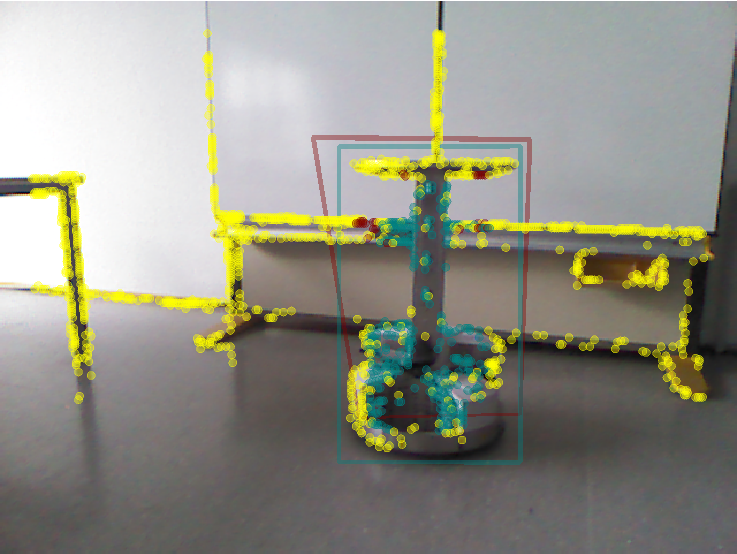
\includegraphics[width=0.7\linewidth]{../media/fo-robo-3}
		\caption{Hier wurde der Robotino durch 2 Templates identifiziert. Das Anwenden von mehreren Templates gleichzeitig erhöht die Fehlerresistenz.}
		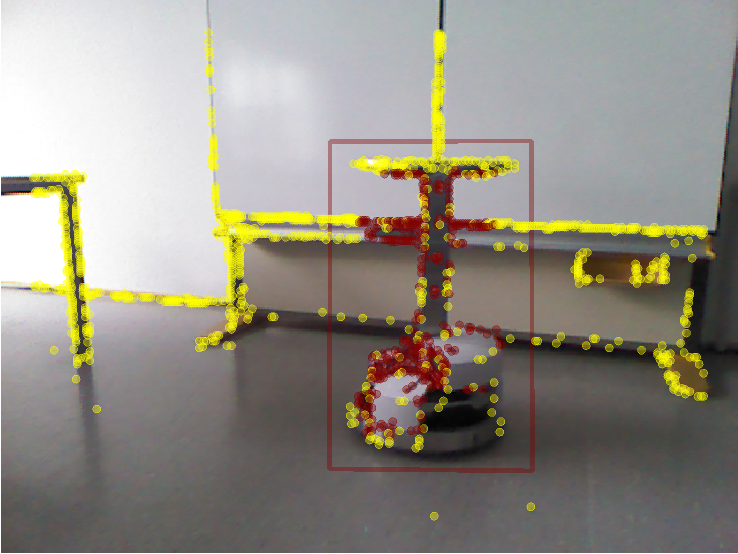
\includegraphics[width=0.7\linewidth]{../media/fo-robotino-1}
		\caption{Hier wurde der Robotino durch 1 Template identifiziert.}
		\label{fig:fo-robo-3}
		\end{figure}

	
%	\begin{itemize}
%	\item Robotino identifizieren Alleinstellungsmerkmal
%	\item Objekt aufnehmen
%	\item spezielles Muster? QR-Code? Abstraktes deutliches schwarz/weiß Design; durch aufbau Form des Robotino nahezu einzigartig
%	\item Wie Perspektivische Unterschiede ausgleichen?
%	\item Roboter von allen Seiten aufnehmen
%	\item je mehr Bilder desto besser;
%	\item Prozess mit Screenshots verdeutlichen
%	\end{itemize}
	Die Unterscheidung zwischen der mobilen Plattform und eines unbekannten Objekts erfolgt durch die Kombination der Objekt-Erkennung und der Identifikation des Robotino. \textit{Find-Object} bietet die Möglichkeit Informationen über identifizierte Objekte in ein dediziertes ROS Topic zu schreiben. Der Informationsgehalt enthält neben der Objekt-ID die Koordinaten des Objekts innerhalb des Frames. Die Abprüfung erfolgt wiederum über einen eigenen ROS-node. Dieser bezieht sich die Koordinaten der mobilen Plattform vom \textit{objects}-Topic, sowie das Differenzbild des \textit{Image\_Subscriber}-Knotens. Nun vergleicht er die Mittelpunkte der Objekte mit den von \textit{Find-Object} ermittelten Koordinaten des Robotinos. Sollten diese Punkte nicht identisch sein handelt es sich nicht um die mobile Plattform sondern um ein Hindernis. Für die Mittelpunktbestimmung werden die Funktionen \textit{find-contours} und \textit{moments} der OpenCV-library genutzt. 

%	\begin{itemize}
%	\item Wie zwischen Objekt und Robotino unterscheiden?
%	\item \textit{Find-Objects} schreibt die identifizierten Objekte in einem Frame in ein eigenes ROS-Topic, objects.
%	\item Durch eigenen Subscriber node die von Find-Objects ermittelten Koordinaten der Plattform innerhalb des Frames mit den Koordinaten der durch sequential images ermittelte Objekte.
%	\item Dazu Einfärben der Objekte mit floodfill Algorithmus = ideal da Kanten der Objekte bekannt.
%	\item liegen die Koordinaten des Robotinos in weißem Bereich des Frames handelt es sich um den Roboter. Ist dies nicht der Fall befindet sich ein Hindernis im Bewegungsraum des Roboters.
%	\end{itemize}
	\subsubsection{floodfill algorithmus}
	Zuerst war der Lösungsansatz für die Objektkoordinatenbestimmung, die mit dem \textit{Image\_Subscriber}-Node detektierten Objkete mit einer eindeutigen Farbe zu füllen. Im nächsten Schritt wurden zufällig Punkte des Frames welche den definierten Farbwert aufweisen, mit den Koordinaten des Robotinos verglichen. Kommt es zu einer Übereinstimmung handelt es sich bei diesem Objekt um die mobile Plattform selbst. Kommt es zu keiner Übereinstimmung befindet sich ein Störobjekt im Bewegungsraum des Roboters.\\ Für das ausfüllen der Objektflächen eignet sich der Floodfill-Algorithmus. Er arbeitet von einem vorgegebenen Startpunkt aus und vergleicht die Farbwerte der Nachbarpunkte mit denen des Startpunktes. Stimmen die Farbwerte des Referenzpunktes und dessen abgeprüften Nachbar überein färbt er beide Punkte mit einer gemeinsamen Farbe ein. Das Voranschreiten im Frame ist abhängig von der Implementierungsweise. Eine Variante hierfür ist das Nutzen eines Stacks. Hierbei werden alle Koordinaten der geprüften Nachbarn in den Stapelspeicher geschrieben. Wurden alle Nachbarn eines Punktes, 4er und 8er Nachbarschaft möglich, geprüft, wird der oberste Eintrag des Stacks als Startwert der nächsten Iteration benutzt. Trifft der Fall zu dass der Farbwert eines Nachbarn nicht mit der des Referenzpunktes übereinstimmt handelt es sich um eine Kante, welche in unserem Fall die Grenze eines Objekts darstellt. In diesem Fall arbeitet der Algorithmus in dieser Richtung nicht mehr weiter, der Punkt wird wieder aus dem Stack genommen und verworfen. Der Fest definierte Startwert des Algorithmus sorgt dafür dass er für den in diesem Projekt erdachten Zweck nicht nutzbar ist. Wenn der Startwert falsch gewählt wird, werden nicht die Flächen der Objekte gefüllt, sondern die Fläche zwischen Ihnen. Dadurch würden keine Störobjekte im Raum identifiziert werden, was zu Kollisionen zwischen fahrender Plattform und Objekten führen kann.\cite{lode-floodfill}
%	\begin{itemize}
%	\item floodfill
%	\item bekommt startpunkt
%	\item prüft benachbarte Punkte auf gemeinsamen Farbwert
%	\item 4er und 8er Nachbarschaft möglich
%	\item Weiterschreiten abhängig von Implementierung
%	\item Stack-variante speichert Koordinaten von Nachbarpunkten in Stapelspeicher, schreitet weiter zum nächsten Pixel per FiLo
%	\item Wenn Nachbar nicht selbe Farbe hat, Kante = Objektgrenze - geht in diese Richtung nicht weiter- Färbt Punkt auch nicht mit definierter Farbe ein.
%	\item Problem besteht darin dass fester Startwert definiert werden muss. Bei dynamischen Objekten nicht anwendbar!
%	\end{itemize}
	
	\newpage
	\subsubsection{find\_contours und moments}	
	Statt der \textit{Floodfill}-Implementierung im OpenCV Paket werden nun die ebenfalls im OpenCV-Paket enthaltenen Funktionen \textit{find\_contours} und \textit{moments} benutzt.
	
	\begin{lstlisting}[caption=imageCallbackV2 Funktion des Objekt-Erkennungs nodes, label=imageCallback-V2, title=imageCallback-V2, language=C++]
	void imageCallback(const sensor_msgs::ImageConstPtr& image)
	{
	sensor_msgs::ImageConstPtr imageInRos;
	imageInRos = image;
	
	cv_bridge::CvImagePtr imageInCV = cv_bridge::toCvCopy(imageInRos);
	
	Mat matNow = imageInCV->image;
	
	
	if(firstrun == 1){
	matMinus1 = matNow;
	firstrun = 0;
	}
	
	///calculate absolute differential and filter noise. Finaly convert to threshold image for improved contrast.
	absdiff(matMinus1, matNow, imageDiff);
	matMinus1 = matNow;
	Mat imageBlur;
	blur(imageDiff,imageBlur,cv::Size(15,15));
	Mat imageThresh;
	threshold( imageBlur, imageThresh, 10, 255,0);
	
	///detect edges
	vector<vector<Point> > contours;
	vector<Vec4i> hierarchy;
	findContours( imageThresh, contours, hierarchy, CV_RETR_EXTERNAL, CV_CHAIN_APPROX_SIMPLE, Point(0, 0) );
	
	///join contours to polygons
	vector<Moments> mu(contours.size() );
	for( int i = 0; i < contours.size(); i++ )
	{ mu[i] = moments( contours[i], true ); }
	
	///calculate the masscenter of each polygon, used as centralpoint of object
	vector<Point2f> mc( contours.size() );
	  for( int i = 0; i < contours.size(); i++ )
	     { mc[i] = Point2f( mu[i].m10/mu[i].m00 , mu[i].m01/mu[i].m00 ); }
	
	///highlight the object-edges and display the masscenter as coloured circle
	Mat drawing = Mat::zeros( imageBlur.size(), CV_8UC3 );
	  for( int i = 0; i< contours.size(); i++ )
	     {
	       Scalar color = Scalar( rng.uniform(0, 255), rng.uniform(0,255), rng.uniform(0,255) );
	       drawContours( drawing, contours, i, color, 2, 8, hierarchy, 0, Point() );
	       circle( drawing, mc[i], 4, color, -1, 8, 0 );
	     }
	
	imshow( "view_contour", drawing );
	imshow("view_mono", matNow);
	imshow("view_diff", imageDiff);
	imshow("view_thresh", imageThresh);
	imshow("view_blur", imageBlur);
	}
	\end{lstlisting}
	
	\begin{itemize}
	\item Zeilen 17, 18, 19: Das Weichzeichnen durch \textit{blur();} wurde vor die Schwellwert-Operation gezogen. hierdurch wird ein besseres Rauschfiltern erreicht.
	\item Block ab Zeile 24: \textit{findcontours} detektiert die Kanten im übergeben Threshold-Bild. Die gefunden Kanten werden in einem Vector-Array gespeichert.
	\item Block ab Zeile 29: Hier werden die detektierten Kanten mittles \textit{moments} zu Polygonen zusammengefügt.
	\item Block ab Zeile 34: Für jedes Polygon wird nun das Massezentrum berechnet, welches als Zentralpunkt des Objekts verwendet wird.
	\end{itemize}
	\cite{cv-findcontours}